\section{Idegsejtek modellezése}



\subsection{Biológiai alapok}
Az idegsejtek magas ion és molekulatartalmú közegben működnek. Legtöbbször a neuron belsejében többlet negatív töltés van, ez felhalmozódik a sejtmembrán belső felületén. A külső felületére pedig az elektromos erők hatására ugyanakkora sűrűségű csak ellenkező előjelű töltés épül fel. A alábbiakban az idegsejtek alapvető biológiai fogalmait tárgyaljuk:

\paragraph{sejtmembrán}
A sejtmembrán egy 3-4 $nm$ vastag kettős lipid réteg, ami lényegében átjárhatatlan a legtöbb töltött molekulára nézve. A sejtmembrán ezen tulajdonsága okozza, hogy tulajdonképpen egy kondenzátorként viselkedik, mivel elkülöníti a belsejében levő és a külső töltéseket.

\paragraph{ioncsatornák}
Számos típusú feszültségfüggő ion-áteresztő csatorna van beleágyazva a sejtmembránba változó sűrűséggel. Ezek bizonyos ionokat átengednek, másokat pedig nem. Részletesebben ezekre nem térünk ki, mert mi csak passzív modellekkel foglalkoztunk vizsgálataink során, aminek az a lényege, hogy a feszültségfüggő csatornákat blokkoljuk és az idegsejt (passzív) viselkedését így vizsgáljuk.

\paragraph{ion pumpák}
Az ion-pumpák tartják fenn hosszútávon a koncentrációgradienst a membrán két oldala között, energiát használva fel.

\paragraph{membránpotenciál}
Konvenció szerint az extracelluláris potenciált rögzítjük nullára. Ennek következtében nyugalomban az idegsejt belseje negatív potenciálú. Az idegsejt akkor van nyugalomban ha a kiáramló és beáramló töltések kioltják egymást. A potenciál úgy változtatható meg, ha kinyitunk vagy bezárunk egy ion-csatornát, illetve ha kísérletileg áramot injektálunk a sejtbe. Mi esetünkben az utóbbit használtuk ki.
A neuron feszültsége átlagos körülmények között $-90 mV$ és $+50 mV$ nagyságrendben mozog, ez teszi lehetővé, hogy az ionok a termális energiát kihasználva átlépjék a membránt. Más nagyságrendet választva nem funkcionálnának az idegsejtek, tehát nem véletlen, hogy a természetes szelekció pont erre az értékre állította be.

A membránpotenciál fontos fogalom az idegsejt leírására, mert annak épp az áramimpulzusra adott feszültségválaszát vizsgáljuk, amiből később következtetéseket vonhatunk le a modell paramétereire.












\subsection{Elektromos tulajdonságok}
Ebben az alfejezetben összefoglaljuk az idegsejtek alapvető elektromos tulajdonságainak a matematikai leírását.

\paragraph{axiális ellenállás}\label{par:Ra}
A kiterjedt idegsejt membránpotenciálja térben általában nem homogén. Ez ion-áramot indít meg a sejt belsejében, ami igyekszik ezt a különbséget kiegyenlíteni. A sejt intracelluláris közege ellenállásként funkcionál erre az áramra nézve (ezért is szokták még intracelluláris ellenállásnak nevezni). Értéke annál nagyobb minél hosszabb és vékonyabb a sejttest (axonok és dendritek esetén például). Két pont között átfolyt áram nagysága könnyen megadható ennek a mennyiségnek és az Ohm törvény segítségével:

\begin{equation}
	I_L = \dfrac{\Delta U}{R_L}
\end{equation}
ahol $\Delta U$ a két pont közötti feszültségkülönbség és $R_L$ pedig a szakasz ellenállása.
$R_L$ arányos a szakasz hosszával és fordítottan arányos a keresztmetszettel. Egy hengeres kábelmodell esetén felírható a következőképpen:
\begin{equation}\label{eq:r_L}
	R_L = \dfrac{R_a L}{\pi a^2}
\end{equation}
ahol $R_a \left[\Omega\cdot cm\right]$ a sejtet jellemző axiális ellenállás (vagy más néven intracelluláris ellenállás, az itteni ábrákon $r_L$ jelöléssel), $a$ pedig a keresztmetszet sugara. A szemléltetés megtalálható a \ref{fig:Ra}-ábrán.

Munkánk során a sejtmodell ezen paraméterét is sokszor becsültük, mivel ez az érték egy jellemzője az idegsejt passzív viselkedésének: a beinjektált áram milyen hatékonyan oszlik szét a sejtben.


\begin{figure}[h!]
	\centering
	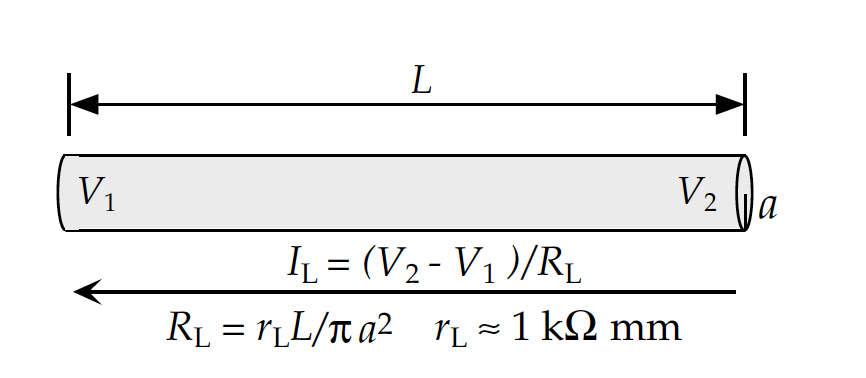
\includegraphics[width=0.5\textwidth]{./fig/Ra.png}
	\caption[Axiális ellenállás]{Az axiális ellenállás szemléltetése egy L hosszúságú kábelszakasz esetén. (Az ábrán $r_L = R_a$ jelölést használunk.) \textit{Forrás:}\cite{dayan2001theoretical} }
	\label{fig:Ra}
\end{figure}


\FloatBarrier
\paragraph{membrán kapacitás}
Fentebb szó volt arról, hogy a membrán úgy viselkedik mint egy kondenzátor. Ebben az esetben az azon felhalmozódó töltést $(Q)$ a következőképp számolhatjuk ki:

\begin{equation}\label{eq:Q}
	Q = C_m V 
\end{equation}
A kapacitás $(C_m)$ azt mondja meg, hogy adott feszültség mellett mennyi töltés halmozódik fel a kondenzátor fegyverzetein, azaz jelen esetben a sejtmembránon. A kapacitás arányos a felülettel, ezért érdemes a membrán tulajdonságait jobban jellemző, felületfüggetlen mennyiséget bevezetni, a specifikus membrán kapacitás:

\begin{equation}\label{eq:cm}
	c_m = \frac{C_m}{A_m}
\end{equation}
ahol $A_m$ a membrán felülete. Ez az érték tipikusan $1 \left[ \dfrac{\mu F}{cm^2}\right]$ nagyságrendbe esik.
Ha idő szerint lederiváljuk a~\ref{eq:Q} egyenlet mindkét oldalát, akkor megkapjuk a membránpotenciál megváltozását adott árambemenetre:

\begin{gather}\label{eq:dV}
	C_m \dfrac{dV}{dt} = \dfrac{dQ}{dt} \\
	\dfrac{dQ}{dt} = I
\end{gather}

\paragraph{membrán ellenállás}
Ahhoz is áram szükséges, hogy a membránpotenciált egy nem egyensúlyi szinten tartsuk. De ezt az áramot már a membrán ellenállás $(R_m)$ határozza meg a kapacitás helyett. Ugyanis Ohm-törvénye értelmében az $I_e$ befecskendezett áram eltolja a membrán potenciált egy $\Delta V$ értékkel:

\begin{equation}\label{eq:Rm}
	\Delta V = R_m I_e
\end{equation}
Ez a képlet csak kis $I_e$ áramok és $\Delta V$ feszültségek esetén érvényes, ha aktív idegsejtről beszélünk, mivel a membrán ellenállás ekkor a feszültség függvénye. Passzív esetben, amikor a membrán ellenállás nem feszültségfüggő, a fenti összefüggés általánosan igaz.
A membrán ellenállás nem más, mint a membrán konduktancia (áteresztőképesség) reciproka, ez pedig hasonlóan a membrán kapacitáshoz arányos a membrán felületével. A passzív membrán konduktancia tehát így írható fel:
\begin{equation}\label{eq:gpas}
	g_{pas} = \dfrac{1}{R_m A} = \dfrac{1}{r_m}
\end{equation}
amelynek tipikus értéke $g_{pas} = 0.0001 \left[\dfrac{\mu S}{cm^2}\right]$ körül mozog.

\paragraph{membrán időállandó}\label{par:tau}
Ha a membránkapacitást és membránellenállást összeszorozzuk akkor egy idő dimenziójú értéket kapunk. Ezt nevezzük a membrán idő állandónak, ami megadja a neurális folyamatok tipikus időskáláját:

\begin{equation}
	\tau_m = C_m R_m \approx \left(10-100\right) \left[ ms \right]
\end{equation}

\paragraph{membránáram}
Ha a membrán összes csatornáján átáramló áramot leosztjuk a membrán felületével, akkor megkapjuk az egységnyi felületre eső membrán áramot $(i_m)$. Passzív idegsejt esetében ez a nem feszültségfüggő (passzív) ion-csatornákból származik. Ezt a jelenséget a membrán passzív konduktanciájával jellemezzük és az ebből fakadó egységnyi felületre eső membránáramot a következőképpen írhatjuk le:

\begin{equation}\label{eq:im}
	i_m = g_{pas}\left( V-E_{pas}\right)
\end{equation}
ahol $g_{pas}$ a membrán passzív áteresztőképessége (konduktanciája) és $E_{pas}$ pedig a megfordítási potenciálja, ami passzív esetben épp az idegsejt nyugalmi potenciálja: $(E_{pas} = V_{m})$. Ezt az értéket meghaladva az ionok ellenkező irányba kezdenek folyni.











\subsection{Egykompartmentumos modell}\label{sec:single-comp}
Egyetlen paraméterrel írjuk le a membránpotenciált, azaz azt tételezzük fel hogy a membrán mentén állandó a potenciálkülönbség. Ez a közelítés egy szómára (egykompartentumos modell) teljesen helytálló, mert könnyen szétterjed benne az áramimpulzus. Tulajdonképpen arról van szó, hogy pontszerűnek tételezzük fel a szómát.
A passzív egykompartmentumos modell leírásához a~\ref{eq:dV} és a \ref{eq:im} egyenleteket kell összerakni:

\begin{equation}\label{eq:one_comp}
	c_m \dfrac{dV}{dt} = -g_{pas} \left( V-E_{pas} \right) + \dfrac{I_e}{A}
\end{equation}
ahol $I_e$ a kísérleti úton sejtbe juttatott áram (stimulus). A \ref{fig:single_comp} ábrán az egykompartmentumos modellek egy általános kapcsolási rajza látható. Vizsgálataink során ennek a modellnek mind a $c_m$ és a $g_{pas}$ (gyakran $g_L$-lel jelölik, mint például az itt fellelhető ábrákon is) paramétereinek az inferenciájával foglalkoztunk.

\begin{figure}[h!]
	\centering
	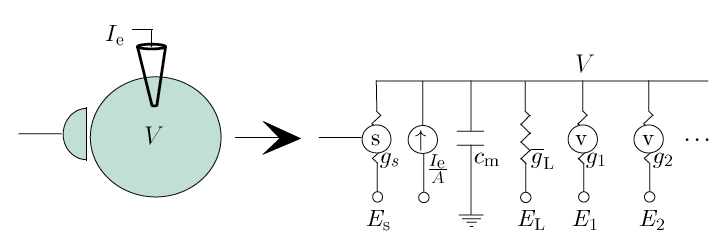
\includegraphics[width=0.7\textwidth]{./fig/single-compartment.png}
	\caption[Egykompartmentumos modell]{Egy általános egykompartmentumos modell, melyen a ion-csatornákból származó és az elektróda áram mellett még egy szinaptikus kapcsolat is van. \textit{Forrás:}\cite{dayan2001theoretical} }
	\label{fig:single_comp}
\end{figure}













\subsection{Térbelileg kiterjedt modellek}\label{sec:multi-comp}
A térbelileg kiterjedt modelleknél már nem tehetjük fel, hogy a membrán mentén a potenciál konstans, térbeli függést is feltételeznünk kell, melyet a kábelegyenlet ír le. Több elemből építjük fel az idegsejtet, melynek az egyes kompartmentumjaiban homogén a potenciál. Minél több részre osztjuk a sejtet, annál részletesebben tudjuk leírni a valós viselkedését. Ezt a folyamatot, vagyis a modellezés különböző szintjeit mutatja be szemléletesen a \ref{fig:multi_comp} ábra. Ez matematikailag összekapcsolt egykompartmentumos modellekkel írható le a következő módon (passzív idegsejt esetén):

\begin{equation}\label{eq:multi_comp}
\begin{split}
		c_m\dfrac{dV_\mu}{dt} = -g_{pas}\left(V_\mu - E_{pas}\right) + \dfrac{I_e^\mu}{A_\mu} + g_{\mu,\mu+1}\left(V_{\mu+1}-V_\mu \right) + g_{\mu,\mu-1}\left(V_{\mu-1}-V_\mu \right)
\end{split}
\end{equation}
ahol $I_e^\mu$ az adott $\mu$-edik kompartmentumba befecskendezett áram, $V_\mu$ a $\mu$-edik kompartmentum membránpotenciálja, $A_\mu$ a $\mu$-edik kompartmentum felülete. Ennek megfelelően $V_{\mu+1}$ és $V_{\mu-1}$ a jelenlegi komparmentumhoz csatlakozó másik kompartmentumok feszültségei. $g_{\mu,\mu+1}$ és $g_{\mu,\mu-1}$ a csatolási tényező, áteresztőképesség a kompartmentumok között, amelyre felírható a következő összefüggés:

\begin{equation}\label{eq:Ra}
	g_{\mu,\mu+1} = \dfrac{a}{2 R_a^{\mu,\mu+1} L^2}
\end{equation}
ahol $R_a$ a \ref{par:Ra}-paragrafusban említett axiális ellenállás, $a$ a kábel keresztmetszetének sugara és $L$ a kábel középpontjait összekötő szakasz hossza, ami ugyanakkora kábeldarabok esetén maga a kábelszakaszok hossza (a képlet erre az esetre érvényes). Inferencia során ezt a paramétert is becsültük, a kompartmentumok között állandónak tekintve ezt az értéket: 
\[ R_a^{\mu,\mu-1} = R_a^{\mu,\mu+1} = ... = R_a \]
Egy ilyen modellnek az általános kapcsolási rajza a \ref{fig:multi_comp_model} ábrán látható. 

Mi egy úgynevezett \textit{Ball and Stick} modellt építettünk vizsgálataink során, ami egy szómához kapcsolódó dendrit esetét reprezentálja. Ezen kívül használtunk egy kísérletből származó, bonyolult térbelileg kiterjedt morfológiát is. 

\begin{figure}[h!]
	\centering
	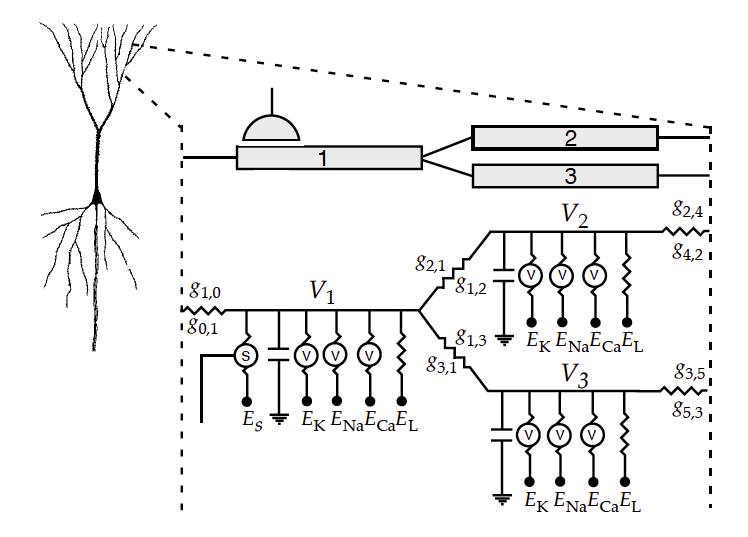
\includegraphics[width=0.7\textwidth]{./fig/multi-comp-model.png}
	\caption[Többkompartmentumos modell]{Egy kiterjedt idegsejt kompartmentumos modelljének kapcsolási rajza. Három kompartmentum látható, az elsőhöz szinaptikus bemenet kapcsolódik. Egy kompartmentumon háromféle ion által keltett áram van jelölve a megfelelő megfordulási potenciálok révén -- melyek feszültségfüggő ellenálláson keresztül kapcsolódnak --, illetve a \textit{"leak"} áram. A membránt pedig a kondenzátor helyettesíti. \textit{Forrás:}\cite{dayan2001theoretical}}
	\label{fig:multi_comp_model}
\end{figure}





\subsection{\textit{NEURON} idegsejt szimulációs program}
A munkánk során a \textit{Python} programozási nyelvet és környezetet használtunk. Az idegsejtek modellezésére, valamint a fentebb tárgyalt egyenletek numerikus megoldására pedig a \textit{NEURON} programot alkalmaztuk. Szerencsére ez betölthető a \textit{Python} környezetébe és így kommunikálni képes vele. Sok különböző paraméterkombinációval végzett szimuláció elvégzésénél ez nagy hasznunkra vált.

A \textit{NEURON} egy szimulációs környezet idegsejtek és komplex hálózatok modellezésére. Kényelmes eszközt szolgáltat modellek építéséhez, kezeléséhez és használatához. Kifejezetten jól alkalmazható esetekhez, melyek szorosan kapcsolódnak kísérleti adatokhoz. A \textit{NEURON "motorja"} különleges algoritmusokat használ annak érdekében, hogy az imént tárgyalt neurális tulajdonságokat leíró egyenleteket, minél hatékonyabban oldja meg. 

Munkánk során mi két modellt építettünk, egy egykompartmentumos -- ami egy neuronból áll -- és egy térbelileg kiterjedt úgynevezett \textit{Ball and Stick} modellt -- ami egy neuronból és egy hozzá csatlakozó dendritből áll. Ezen kívül egy valós kísérletből származó anatómiailag részletes modellre is alkalmaztuk megoldásainkat, melynek \textit{NEURON}-ba töltött rekonstrukciója látható a \ref{fig:morph}-ábrán.

\begin{figure}[h!]
	\centering
	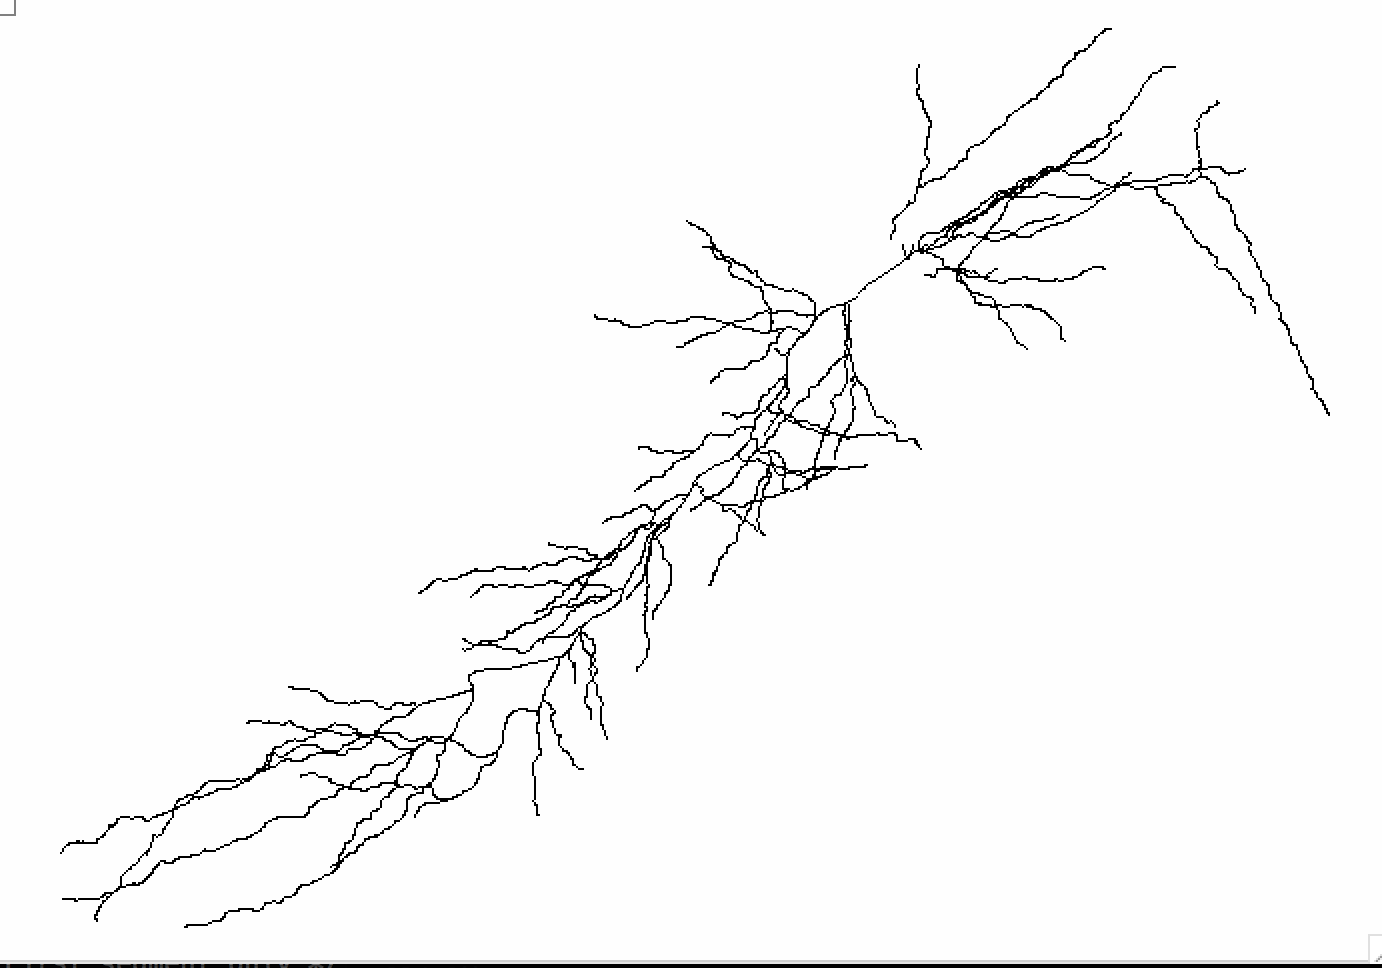
\includegraphics[width=0.5\textwidth]{./fig/morph.png}
	\caption[Kísérletből származó morfológia]{Egy valós idegsejt \textit{NEURON} programba töltött modellje.}
	\label{fig:morph}
\end{figure}


Az összes általunk használt modellt passzív idegsejti mechanizmus mellett vizsgáltuk. Ez azt jelenti, hogy az áramimpulzus hatására nem \textit{"tüzel"} az idegsejt, csak passzívan folyik belsejében az áram. Kísérletileg ezt bonyolult módon csatorna blokkolókkal lehet elérni, \textit{NEURON}-ban csupán beállítás kérdése.

Korábban láttuk, hogy hogyan is modellezünk egy biológiailag nagyon komplex idegsejtet: egyszerű elektronikából ismert hálózati elemekből összerakott modell nagyon jól visszaadja az empirikus megfigyeléseket. Ezek a vezetőképességen alapuló modellek az idegsejteknek a lehetséges legegyszerűbb biofizikai reprezentációi, melyekben az ion csatornákat ellenállásokkal, illetve a kettős lipid membránt pedig egy kapacitással helyettesítik (egy ilyen látható a~\ref{fig:fig1}. ábrán). Illetve az idegsejtet részegységekre (kompartmentumokra) bontjuk, melyek egy csatolt differenciál-egyenletrendszert szolgáltat. Az idegsejt ilyen jellegű modellezése, azaz kompartmentumos leírása látható a \ref{fig:multi_comp} ábrán. Analitikusan az idegsejt felosztásával tarthatunk a nullába, viszont numerikusan ez nem megoldható, véges kompartmentumokkal közelítünk.

\begin{figure}[h!]
	\centering
	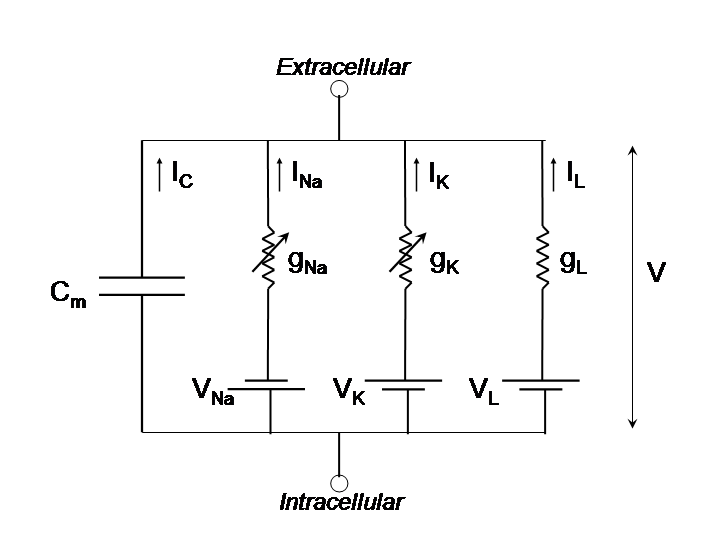
\includegraphics[width=0.6\textwidth]{./fig/Fig1.png}
	\caption[Idegsejt modell]{Példa az idegsejt konduktancián alapuló kapcsolási modelljéről. \\ \href{http://www.scholarpedia.org/w/images/e/eb/Fig1.png}{\textit{Forrás: http://www.scholarpedia.org/w/images/e/eb/Fig1.png}}}
	\label{fig:fig1}
\end{figure}

\begin{figure}[!h]
	\centering
	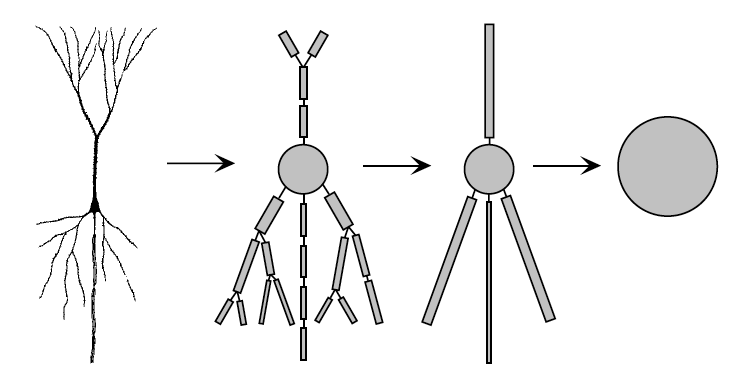
\includegraphics[width=0.6\textwidth]{./fig/multi-compartment.png}
	\caption[Többkompartmentumos modellezés]{\cite{dayan2001theoretical} Egy idegsejt különböző szintű kompartmentális modellezése. Jobbra haladva egyre inkább leegyszerűsítve írjuk le a sejtet.}
	\label{fig:multi_comp}
\end{figure}


